% Use preinstalled Times-compatible fonts for the local XeTeX build.
% Other engines retain IEEEtran's standard font setup.
\ifdefined\XeTeXversion
\IfFileExists{/usr/share/fonts/gsfonts/NimbusRoman-Regular.otf}{%
  \DeclareFontFamily{TU}{ptm}{}
  \DeclareFontShape{TU}{ptm}{m}{n}{<->"[/usr/share/fonts/gsfonts/NimbusRoman-Regular.otf]:mapping=tex-text"}{}
  \DeclareFontShape{TU}{ptm}{m}{it}{<->"[/usr/share/fonts/gsfonts/NimbusRoman-Italic.otf]:mapping=tex-text"}{}
  \DeclareFontShape{TU}{ptm}{b}{n}{<->"[/usr/share/fonts/gsfonts/NimbusRoman-Bold.otf]:mapping=tex-text"}{}
  \DeclareFontShape{TU}{ptm}{b}{it}{<->"[/usr/share/fonts/gsfonts/NimbusRoman-BoldItalic.otf]:mapping=tex-text"}{}
  \DeclareFontShape{TU}{ptm}{bx}{n}{<->ssub*ptm/b/n}{}
  \DeclareFontShape{TU}{ptm}{bx}{it}{<->ssub*ptm/b/it}{}
  \DeclareFontShape{TU}{ptm}{m}{sc}{<->ssub*ptm/m/n}{}
  \DeclareFontFamily{TU}{pcr}{}
  \DeclareFontShape{TU}{pcr}{m}{n}{<->"[/usr/share/fonts/gsfonts/NimbusMonoPS-Regular.otf]:mapping=tex-text"}{}
}{}
\fi

\documentclass[conference]{IEEEtran}
\usepackage{mathptmx}
\usepackage{amsmath,amssymb,booktabs,cite,url,graphicx}
\usepackage{tikz}
\usetikzlibrary{positioning,arrows.meta}
\usepackage[hidelinks]{hyperref}
\setlength{\emergencystretch}{2em}
\makeatletter
\newcommand{\linebreakand}{\end{@IEEEauthorhalign}\hfill\mbox{}\par\vspace{1em}\mbox{}\hfill\begin{@IEEEauthorhalign}}
\makeatother
\renewenvironment{abstract}{\par\noindent\normalfont\normalsize\textbf{Abstract.}\enspace\ignorespaces}{\par\vspace{0.6\baselineskip}}
\renewenvironment{IEEEkeywords}{\par\noindent\normalfont\small\textit{Index Terms:}\enspace\ignorespaces}{\par\vspace{0.6\baselineskip}}
\IEEEtriggeratref{11}
\title{@TITLE@}
\author{@AUTHORS@}
\begin{document}
\maketitle

\begin{abstract}
Jevlet uses a shared DistilBERT encoder to return a single label, a five-level sentiment rating, a yes/no answer, or a set of labels. We extend its original three-head interface with separate emotion and banking multi-label heads. Each new head scores option-marker representations with independent sigmoids and learns through masked binary cross-entropy. Sequential CPU fine-tuning uses human-annotated GoEmotions and NLU++ banking data, with replay examples from earlier tasks. We calibrate probabilities on held-out data and select thresholds on validation data. Given shortlists of two to ten labels, the emotion checkpoint reaches @EMOTION_MICRO@\% micro-F1 on 768 test texts, compared with @EMOTION_BASELINE_MICRO@\% for TF-IDF logistic classifiers. The combined checkpoint reaches @BANK_MICRO@\% banking micro-F1 on 204 test messages, compared with @BANK_BASELINE_MICRO@\% for its matched baseline. We also report set accuracy, per-label and aggregate performance, probability calibration, and earlier-task checks on matched examples. These single-seed results measure decisions within supplied lists; full-catalogue retrieval, unrestricted question understanding, and confidence reliability in production remain untested.
\end{abstract}
\begin{IEEEkeywords}
shared encoder, multi-label classification, typed text decisions, banking intent detection, emotion recognition, probability calibration
\end{IEEEkeywords}

\section{Introduction}
A customer who writes that a transfer is not working describes both an action and a problem. Similarly, a short comment may express gratitude and joy together. Selecting one label loses part of the meaning in either case. Other questions do require a single answer, such as one banking intent, a sentiment level from one to five, or a yes/no decision. A text-processing interface needs to specify which kind of answer each question allows.

Jevlet combines a text context, typed questions, and candidate labels in one sequence. A single DistilBERT pass produces representations at question and option markers; task-specific heads then produce structured answers. The original model handles banking shortlist selection, review sentiment, and binary intent questions. We extend it with separate multi-label scorers trained on GoEmotions emotion labels and NLU++ banking intent components. Because these scorers do not normalize probabilities across candidates, several labels can receive high probabilities in the same answer.

We contribute a five-head interface and a reproducible procedure for extending it in stages using released multi-label annotations. Each task has its own probability calibration, and each multi-label head has its own decision threshold. The evaluation measures both candidate coverage and prediction quality within the supplied lists. We also check earlier tasks on matched examples and provide a local dashboard for inspecting predictions. Our experiments cover a supervised English-text workload.

We use stage E to denote the emotion extension and stage B to denote the subsequent banking extension, which retains the emotion head. An archived three-head GPU experiment provides a separate comparison. These settings use different datasets, checkpoint histories, and metric definitions, so we report their results separately.

\section{Background and Related Work}
\subsection{Encoders and Label Representations}
BERT introduced bidirectional transformer representations for downstream language tasks~\cite{bert}. DistilBERT provides a smaller encoder through knowledge distillation~\cite{distilbert}. Jevlet fine-tunes DistilBERT and its output heads without an additional distillation step. We also consider RoBERTa and sparse linear classifiers as comparison models~\cite{roberta,svm}. Laya's typed interface and marker scoring informed our implementation~\cite{laya}. Although Jevlet accepts question text, its ability to answer arbitrary questions or generalize to unseen labels has not been established.

Wang et al.'s label-embedding attentive model (LEAM) learns compatible word and label representations and uses their attention scores to represent text~\cite{leam}. Jevlet also conditions predictions on label text, but places question and option markers in a shared transformer sequence and scores the contextualized markers. The connection concerns how labels enter the model; our experiments do not compare Jevlet with LEAM or establish transfer to new label meanings.

\subsection{Multi-Label Prediction and Data}
Zhang and Zhou review multi-label methods, including binary relevance and approaches that model label correlations~\cite{multilabel_review}. Jevlet's multi-label heads make separate binary decisions after shared contextual encoding. Yang et al.'s sequence generation model instead predicts a label sequence to capture label correlations~\cite{sgm}. Jevlet has no sequential label decoder or explicit joint distribution over label sets. Comparing these approaches would require a matched experiment with the same data and candidate lists.

BANKING77 assigns one fine-grained banking intent to each message, and SST-5 assigns one ordered sentiment label to each review~\cite{banking,sst}. Deriving several binary questions from a BANKING77 label supplies supervision for multiple tasks, but does not create a human-annotated multi-label intent set. GoEmotions supplies such annotations for emotions that co-occur in English comments~\cite{goemotions}. NLU++ combines generic and domain-specific intent modules in task-oriented messages, including banking messages~\cite{nlupp}. Its modules do not map directly to BANKING77's 77 classes.

\subsection{Task Sharing and Replay}
Sharing an encoder makes task balancing relevant. GradNorm adapts task weights through gradient magnitudes~\cite{gradnorm}, while PCGrad projects conflicting task gradients~\cite{pcgrad}. Jevlet averages losses across active heads and does not implement either method. They offer concrete alternatives for investigating task interference, whose cause is not identified by our retention checks alone.

De Masson d'Autume et al. combine sparse experience replay with local adaptation in lifelong language learning~\cite{episodic_memory}. Our staged training reuses earlier examples, but uses fixed replay subsets and no inference-time local adaptation. We evaluate retention on matched examples without claiming to reproduce their continual-learning protocol or eliminate forgetting.

\subsection{Objectives, Calibration, and Thresholds}
The original sentiment head uses ordered cumulative prediction~\cite{coral}; an earlier comparison also evaluates a categorical head. Asymmetric Loss downweights easy negative examples to address positive--negative imbalance in multi-label image classification~\cite{asymmetric_loss}. It is a possible alternative to our masked binary cross-entropy and Brier penalty; its benefit for these text tasks has not been tested.

We use temperature scaling and Brier error to study probability quality~\cite{guo,brier}, with calibration assessed only on the evaluated domains. Lipton et al. analyze how F1 optimization depends on the decision threshold~\cite{f1_threshold}. This motivates treating probability fitting and label-set selection separately. We fit temperature to calibration NLL, then select a threshold by validation micro-F1. This procedure does not guarantee optimal F1 on a new test distribution.

\section{Typed Shared-Encoder Architecture}
\subsection{Input Contract and Packing}
Each request contains a text $x$ and one to three typed questions $Q$. Choice and multi-label questions also supply two to ten distinct candidate strings. We pack the input as
\begin{equation}
[\mathrm{CLS}]\;B(Q)\;[\mathrm{SEP}]\;x\;[\mathrm{SEP}],
\end{equation}
where $B(Q)$ places a learned \texttt{[Q]} marker before each question and a learned \texttt{[OPT]} marker before each candidate. The tokenizer records their positions. Reserved marker strings in user text cannot introduce additional model markers.

The sequence has a 256-token budget. Questions and candidates take priority, with the remaining tokens available for context. The context is truncated when necessary, and inference reports how many context tokens were removed. A question block that leaves no room for context is rejected. Padding and candidate masks identify unused positions. A longer shortlist can cover more labels, but leaves less room for the text.

DistilBERT-base has six transformer layers, a hidden dimension of 768, and twelve attention heads. We gather its contextual representations at question markers, $h_q$, and option markers, $h_{o_j}$. Self-attention allows these representations to depend on the questions, candidates, and context together. The final checkpoint has five task output heads (Fig.~\ref{fig:architecture}); its predecessors have three or four. These output heads are separate from the encoder's attention heads.

\begin{figure*}[!t]
\centering
\resizebox{0.98\textwidth}{!}{%
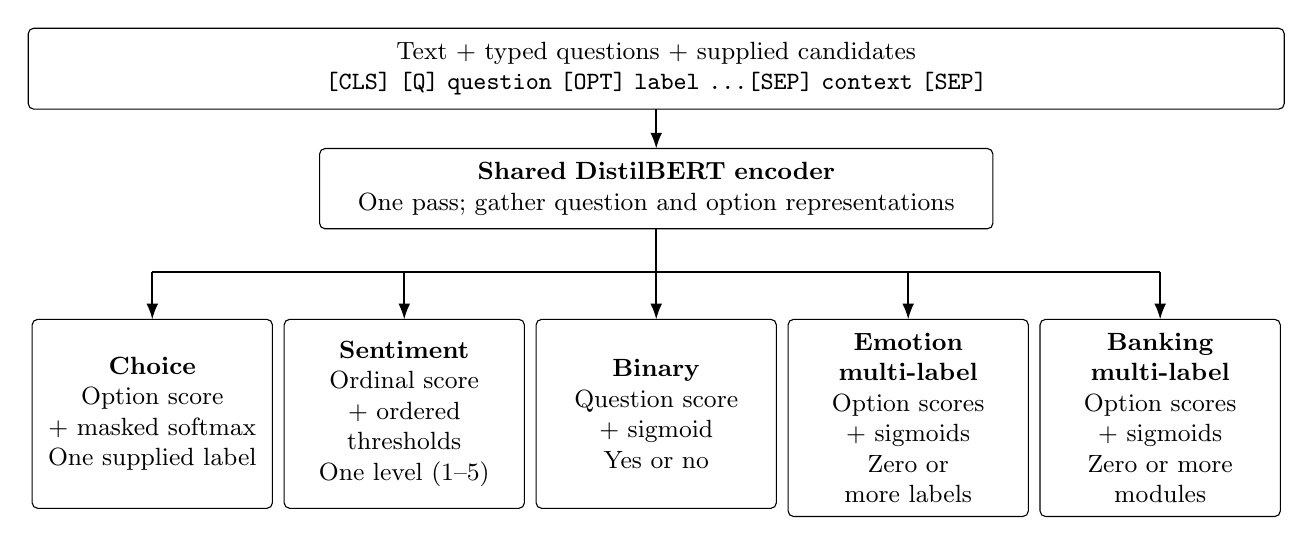
\begin{tikzpicture}[
  box/.style={draw,rounded corners=2pt,align=center,inner sep=5pt,outer sep=0pt,font=\small},
  head/.style={box,anchor=north,text width=2.7cm,minimum height=2.4cm},
  flow/.style={-{Latex[length=2mm]},semithick}]
\node[box,anchor=south,text width=8.2cm,minimum height=1cm] (encoder) at (0,1.15) {\textbf{Shared DistilBERT encoder}\\One pass; gather question and option representations};
\node[box,above=0.50cm of encoder,text width=15.6cm,minimum height=0.9cm] (input) {Text + typed questions + supplied candidates\\\texttt{[CLS] [Q] question [OPT] label \ldots [SEP] context [SEP]}};
\node[head] (choice) at (-6.4,0) {\textbf{Choice}\\Option score\\+ masked softmax\\One supplied label};
\node[head] (score) at (-3.2,0) {\textbf{Sentiment}\\Ordinal score\\+ ordered thresholds\\One level (1--5)};
\node[head] (binary) at (0,0) {\textbf{Binary}\\Question score\\+ sigmoid\\Yes or no};
\node[head] (emotion) at (3.2,0) {\textbf{Emotion multi-label}\\Option scores\\+ sigmoids\\Zero or more labels};
\node[head] (banking) at (6.4,0) {\textbf{Banking multi-label}\\Option scores\\+ sigmoids\\Zero or more modules};
\draw[flow] (input)--(encoder);
\draw[semithick] (encoder.south)--(0,0.6);
\draw[semithick] (-6.4,0.6)--(6.4,0.6);
\foreach \x/\name in {-6.4/choice,-3.2/score,0/binary,3.2/emotion,6.4/banking} {\draw[flow] (\x,0.6)--(\name.north);}
\end{tikzpicture}}
\caption{Five task heads share one encoder. Each head has its own temperature, and each multi-label head has its own selection threshold. A request uses only the answer types it specifies. The final checkpoint uses ordinal sentiment; the categorical variant was evaluated in an earlier experiment.}
\label{fig:architecture}
\end{figure*}

\subsection{Single-Choice, Binary, and Sentiment Outputs}
For a choice question, one shared linear scorer assigns each supplied option a logit $z_j=w_c^\top h_{o_j}+b_c$. A masked softmax produces probabilities that sum to one over the candidate list. Argmax selects one label, regardless of how many candidates are supplied.

The binary head applies a sigmoid to the question-marker score. The probability of no is the complement of the probability of yes. For ordinal sentiment, the head learns a scalar score $s$ and four thresholds $\beta_1<\cdots<\beta_4$, ordered through positive softplus increments. With $u_k=\sigma((s-\beta_k)/T_s)$, the five class probabilities are $(1-u_1,u_1-u_2,u_2-u_3,u_3-u_4,u_4)$. The output includes the most probable level and the expected rating. An optional categorical head uses five softmax logits. Both CPU extension stages inherit the ordinal head from the initial CPU checkpoint; the categorical checkpoint selected in the earlier GPU experiment is a separate model.

\subsection{Two Multi-Label Heads}
For emotion and banking multi-label prediction, indexed by $d\in\{e,b\}$, separate linear scorers assign a logit and probability to each option:
\begin{equation}
z_{dj}=w_d^\top h_{o_j}+b_d,\qquad
p_{dj}=\sigma(z_{dj}/T_d).
\end{equation}
Applying the task-specific threshold gives the selected set
\begin{equation}
\widehat{Y}_d=\{c_j\in C:p_{dj}\geq\tau_d\},
\end{equation}
where $C$ is the supplied candidate list. These probabilities need not sum to one. Each scorer adds 769 learned parameters for a 768-dimensional input. Self-attention can capture interactions between labels, although the sigmoid outputs do not define an explicit joint distribution over label sets.

A multi-label answer can contain zero, one, or several labels. An empty answer means that no supplied candidate met the threshold. We have not validated it as a way to detect out-of-domain inputs. The model also does not assign a confidence score to the correctness of the whole set by taking the largest label probability. GoEmotions' Neutral is an annotated label and can be selected like any other; it is distinct from an empty answer. NLU++ modules describe actions, objects, and states, with meanings that differ from BANKING77 classes. The model does not extract slots.

\section{Supervision, Calibration, and Selection}
\subsection{Masked Multi-Label Objective}
The multi-label target is a binary vector over the supplied candidates, with $-1$ marking an explicitly unknown annotation. For observed positions $O$, we minimize
\begin{align}
\ell_d={1\over|O|}\sum_{j\in O}\big[&-y_j\log p_j-(1-y_j)\log(1-p_j)\nonumber\\
&+\lambda(p_j-y_j)^2\big],\qquad\lambda=0.5.
\end{align}
During training, $T_d=1$ and binary cross-entropy is computed directly from logits. We exclude padding and unknown annotations from both loss and evaluation decisions. The experiments treat the released label sets as complete annotations. The implementation supports partial annotations, but we do not introduce a new partially annotated dataset.

Choice and categorical sentiment use cross-entropy, while binary and ordinal cumulative targets use binary cross-entropy. Their Brier penalties sum over class probabilities. The multi-label Brier penalty averages squared error over observed binary decisions, so its scale differs from the multiclass penalties. We average question losses within each active task head, then average across those heads. Training updates the full encoder and the active heads.

\subsection{Probability Fitting and Set Thresholds}
After checkpoint selection, we fit one positive temperature per task on the calibration partition by minimizing negative log-likelihood (NLL). For multi-label tasks, binary NLL is computed over observed candidate positions. L-BFGS optimizes a bounded log-temperature. All labels handled by a head share this temperature, including rare labels.

We then select each multi-label threshold by maximizing validation micro-F1 over a grid from 0.05 to 0.95 in steps of 0.01. Ties favor the threshold closest to 0.5. Stage E selects an emotion threshold of @EMOTION_THRESHOLD@. Stage B selects @FINAL_EMOTION_THRESHOLD@ for emotion and @BANK_THRESHOLD@ for banking. Test data is excluded from weight, temperature, and threshold selection. Checkpoint and threshold selection reuse the validation partition; this is not nested validation, and we do not estimate the uncertainty introduced by that reuse.

\subsection{Implemented Question-Refinement Workflow}
The implementation supports five paraphrase templates for each original choice, binary, and sentiment question. It can expand validation to five correlated views while keeping a request seed fixed across training seeds. A separate CUDA workflow ranks refinement candidates by sentiment accuracy on expanded validation, subject to banking-performance guardrails. The CPU multi-label runs use a simpler protocol: one canonical validation view and checkpoint selection by validation loss. Repeated views of the same text would add neither independent examples nor cross-validation folds.

\section{Data and Experimental Protocol}
\subsection{Released Multi-Label Data}
For stage E, we select a deterministic subset of the simplified GoEmotions release, retaining the separation between its original training and test partitions. Before selection, we remove repeated source IDs and duplicate texts after case folding and whitespace normalization, giving test examples priority. We deterministically shuffle the official development data and assign alternating examples to validation and calibration. The training subset contains all 28 labels. Table~\ref{tab:partitions} lists the resulting partition sizes.

\begin{table}[!t]
\caption{Primary multi-label partition sizes after filtering, excluding replay}
\label{tab:partitions}
\centering\footnotesize\setlength{\tabcolsep}{3.5pt}
\begin{tabular}{lrrrrr}\toprule
Dataset & Labels & Train & Valid. & Cal. & Test\\\midrule
GoEmotions E & 28 & 4,096 & 384 & 384 & 768\\
NLU++ banking B & 48 & 1,422 & 206 & 207 & 204\\\bottomrule
\end{tabular}
\end{table}

Stage B uses the 48 generic and banking modules in the official NLU++ ontology. Source folds 0--13 form the training partition, 14--15 validation, 16--17 calibration, and 18--19 test. When a text occurs in more than one partition, we retain it in the first partition in the order test, calibration, validation, training. We use this single fixed split rather than the repeated low-, mid-, or large-data cross-validation protocol of the NLU++ paper. The examples retain their released human annotations; we do not create synthetic combinations of messages.

The evidence manifest records the pinned dataset revisions: \texttt{add492243ff9\ldots} for GoEmotions and \texttt{57ec275d8078\ldots} for NLU++, along with hashes of every NLU++ source-fold file. GoEmotions is licensed under Apache-2.0 and NLU++ under CC-BY-4.0. Their source-data obligations still apply when model artifacts are released.

\subsection{Candidate Construction and Coverage}
We construct candidates separately within each source partition. A deterministic sampling procedure chooses among three modes: include all true labels, include one true label, or include no true labels, with weights 0.70, 0.15, and 0.15. For texts with one true label, the first two modes include the same positives. Randomly sampled non-gold labels fill the remaining positions. Each list contains two to ten candidates and has enough room for the included positives. Omitting a true label from a shortlist does not change the released annotation.

This procedure uses gold annotations to construct shortlists; it does not train a candidate retriever. Candidate recall measures the fraction of annotated true labels present in those lists. Recall is 0.8236 on the 768 emotion texts and 0.7093 on the 204 banking messages. Neither Jevlet nor the baseline can recover a label absent from its input list. We therefore define exact-set accuracy over the observed labels \emph{within that list}, rather than over all annotated labels in the full catalogue.

\subsection{Sequential Fine-Tuning and Replay}
We start from the CPU-trained three-head Jevlet checkpoint, supervised on BANKING77 and SST-5. Stage E initializes an emotion scorer from the choice scorer and trains for three epochs. Each epoch includes 4,096 emotion texts, 64 BANKING77 replay texts, and 64 SST-5 replay texts. Stage B starts from stage E, initializing its separate banking scorer from the emotion scorer. It also trains for three epochs, each containing 1,422 NLU++ messages plus 64 BANKING77, 64 SST-5, and 256 emotion replay texts. The two stages thus process 4,224 and 1,806 requests per epoch before packing.

Both stages use seed 42 and AdamW with a learning rate of $3\times10^{-5}$, weight decay of 0.01, and 10\% linear warm-up. The batch size is eight, with two-step gradient accumulation and gradient clipping at one. Training runs in float32 on CPU using four PyTorch threads; the saved mixed-precision option has no effect on CPU. Validation loss is lowest at epoch three in both runs, so we select those checkpoints. Calibration and test batches contain up to 32 requests. The runs use PyTorch 2.14.1+cpu, Transformers 4.57.6, scikit-learn 1.9.1, and NumPy 2.4.6.

Stage B includes up to 128 emotion replay texts in each held-out partition. An audit found that one emotion-calibration replay text also appeared in banking training. We removed the calibration copy, leaving 127 emotion calibration texts, and recomputed calibration, thresholds, and evaluation. Trained weights and the training, validation, and test manifests stayed fixed. After this correction, the combined partitions share no texts. NLU++ test texts also have no exact normalized matches in either ancestor checkpoint's recorded training texts. This audit checks exact text overlap; paraphrase overlap and overlap with unsupervised encoder pretraining remain possible.

\subsection{Matched Baseline and Metrics}
The baseline fits unigram and bigram TF-IDF features on training contexts only, with a limit of 20,000 features. It trains one regularized logistic classifier per label using all known positive and negative annotations for that label. Where class variation is insufficient, a smoothed training prior replaces the classifier. We fit the baseline's own temperatures and thresholds using the same calibration and validation roles as Jevlet. Both systems receive identical test texts, candidate lists, and binary targets, although their feature representations and training objectives differ.

Micro-F1 pools observed candidate decisions. Macro-F1 averages per-label F1 over labels that appear in the supplied lists, assigning zero to undefined divisions. Precision and recall are pooled as well. We also measure exact candidate-set accuracy, Hamming loss, binary NLL, mean per-decision Brier error, and calibration error with 15 bins of positive-label probabilities. Exact-set accuracy excludes partially annotated examples. Single-choice accuracy, sentiment MAE, and binary-predicate accuracy describe the original tasks and are reported separately.

\section{Results and Discussion}
\subsection{Multi-Label Quality}
Stage E reaches @EMOTION_MICRO@\% micro-F1, compared with @EMOTION_BASELINE_MICRO@\% for TF-IDF, a gain of @EMOTION_DELTA@ percentage points (Table~\ref{tab:multilabel}). Stage B reaches @BANK_MICRO@\% banking micro-F1 against @BANK_BASELINE_MICRO@\%, a gain of @BANK_DELTA@ points. These are single-seed differences, so they do not estimate variability across training seeds. The two domains also differ in label meanings, prevalence, candidate lists, and test size. Comparing their F1 values does not establish which task is harder.

\begin{table*}[!t]
\caption{Multi-label test results for supplied candidate lists. F1, precision, recall, exact-set accuracy, and Hamming loss are proportions. Exact-set accuracy measures agreement within the supplied list.}
\label{tab:multilabel}
\centering\footnotesize\setlength{\tabcolsep}{4.5pt}
\begin{tabular}{llrrrrrrr}\toprule
Task & Configuration & Texts & Micro-F1 & Macro-F1 & Precision & Recall & Exact & Hamming\\\midrule
@MULTILABEL_ROWS@
\bottomrule\end{tabular}
\end{table*}

The gap between micro- and macro-F1 is larger for emotion than for banking. Label support is uneven, with few positive examples for some rare classes. The saved metrics include per-label counts, which are needed to assess performance beyond the averages. In particular, the aggregate scores do not show that all emotions or banking modules are recognized equally well. TF-IDF remains competitive on NLU++, making it a useful reference when weighing the extra cost of contextual marker representations.

\begin{table}[!t]
\caption{Calibrated multi-label probabilities and candidate recall}
\label{tab:probability}
\centering\scriptsize\setlength{\tabcolsep}{3pt}
\begin{tabular}{llrrrr}\toprule
Task & Model & Brier & NLL & ECE & Cand. recall\\\midrule
@PROBABILITY_ROWS@
\bottomrule\end{tabular}
\end{table}

The calibrated probability results appear in Table~\ref{tab:probability}. Expected calibration error (ECE) measures individual positive-label probabilities, not confidence in the correctness of a whole predicted set. Sharing one temperature per head keeps the number of fitted parameters small, but cannot correct every label-specific error. We fit temperature to held-out NLL, so the procedure need not minimize test ECE or F1, or improve every metric after a distribution shift.

\subsection{Matched Earlier-Task Checks}
The final checkpoint's emotion evaluation contains 128 texts, compared with 768 in the primary stage-E evaluation. To compare the checkpoints on the same data, we locate those 128 source IDs in the saved stage-E predictions, verify that their candidates and targets match, and recompute the metrics (Table~\ref{tab:emotionretention}). Each checkpoint uses its own calibration and validation-selected threshold. The comparison therefore measures changes in the full prediction procedure; it cannot isolate the effect of banking-training gradients. On this subset, micro-F1 rises while macro-F1 falls. These mixed results do not establish full retention of earlier-task quality.

\begin{table}[!t]
\caption{Emotion results on identical texts and candidate lists}
\label{tab:emotionretention}
\centering\footnotesize\setlength{\tabcolsep}{4pt}
\begin{tabular}{lrrrr}\toprule
Checkpoint & Texts & Micro-F1 & Macro-F1 & Exact\\\midrule
@EMOTION_RETENTION_ROWS@
\bottomrule\end{tabular}
\end{table}

We also compare the original tasks using the same held-out source IDs and derived questions (Table~\ref{tab:legacyretention}). Between stages E and B, choice and sentiment each incur one additional error among 64 texts per task. Binary prediction incurs three additional errors among 128 predicates. The replay examples keep the tasks available, but do not prevent all regressions. These small subsets cannot establish non-inferiority on the full test sets.

\begin{table}[!t]
\caption{Original-task accuracy on matched examples (percent)}
\label{tab:legacyretention}
\centering\footnotesize\setlength{\tabcolsep}{4pt}
\begin{tabular}{lrrr}\toprule
Checkpoint & Choice (64) & Sentiment (64) & Binary (128)\\\midrule
@LEGACY_RETENTION_ROWS@
\bottomrule\end{tabular}
\end{table}

\subsection{Archived GPU Comparison}
The archived three-head GPU experiment at repository revision \texttt{38ed101} evaluated 3,079 choice, 2,210 sentiment, and 6,158 binary decisions from the full retained BANKING77/SST-5 test data (Table~\ref{tab:historical}). We have not rerun or independently re-audited those measurements for this extension. They provide historical context for the original heads; they do not measure five-head inference or multi-label performance.

\begin{table}[!t]
\caption{Three-head results from the separate archived GPU experiment}
\label{tab:historical}
\centering\scriptsize\setlength{\tabcolsep}{2.5pt}
\begin{tabular}{lrrrr}\toprule
Configuration & Choice \% & Sent. \% & Sent. F1 & Binary \%\\\midrule
@HISTORICAL_ROWS@
\bottomrule\end{tabular}
\end{table}

In the archived experiment, categorical Jevlet reaches 52.22\% sentiment accuracy, compared with 35.20\% for ordinal Jevlet and 54.12\% for RoBERTa. This result motivates considering a categorical sentiment head. The final CPU checkpoint still uses an ordinal head, so the categorical model's 52.22\% accuracy does not describe it. Nor are these full-test scores directly comparable with the 64-text checks. Further CUDA refinement and expanded validation belong to a separate workflow from the CPU multi-label stages.

\subsection{Training Cost and Local Demonstration}
The recorded CPU training intervals include training, validation, and checkpoint saving (Table~\ref{tab:training}). They exclude initial preparation, calibration, and test evaluation. Because the stages differ in data size and starting checkpoint, the intervals do not compare models under equal compute budgets. We have not run systematic latency or concurrent-load benchmarks for the new multi-label heads. Individual browser-call timings cannot establish an architectural speedup.

\begin{table}[!t]
\caption{CPU training time and final-epoch losses}
\label{tab:training}
\centering\footnotesize\setlength{\tabcolsep}{3.5pt}
\begin{tabular}{lrrrr}\toprule
Stage & Minutes & Epochs & Train loss & Valid. loss\\\midrule
@TRAINING_ROWS@
\bottomrule\end{tabular}
\end{table}

The local dashboard loads the trained checkpoint and provides five examples: single-choice banking, review sentiment, confidence-based routing, multi-label emotion, and multi-label banking. It displays model probabilities and task-specific thresholds. Adjusting a multi-label threshold reuses the most recent probability vector. For ``I am trying to make a transfer but it is not working'', the banking head selects the action, transfer/payment, and not-working modules. The display uses readable label titles, while requests and responses retain the dataset's catalogue values.

The CPU suite reports 61 passing tests for source-fold isolation, annotation masks, five-head training and save/reload, separate calibration, fixed request seeds, and refinement compatibility. Browser checks with the trained checkpoint cover all five examples on desktop and mobile, including truncation, candidate edits, and visible error recovery. These checks verify implementation and browser behavior. The routing example previews a policy whose operational effectiveness has not been evaluated.

\section{Limitations and Reproducibility}
Each extension uses one seed and one fine-tuning schedule, and the checkpoints share a training history. We therefore cannot assess robustness across random initializations, identify an optimal replay policy, or attribute gains to individual architectural components. Repeated-seed training and fresh full-test evaluations of earlier tasks are needed. The small NLU++ test set and limited support for rare labels further restrict generalization. Our fixed split also differs from the dataset authors' cross-validation benchmark.

The evaluation assumes that candidate lists are supplied and released annotations are complete. Constructing lists from gold annotations, including cases with omitted true labels, lets us examine decisions under known candidate coverage. It does not validate a production candidate generator: the model can return only labels in the supplied list. Set accuracy, candidate recall, and probability calibration measure different aspects of this process and need to be considered together. We have not established transfer to unseen labels, arbitrary rubrics, multilingual text, slot extraction, or out-of-domain detection.

Sharing an encoder can cause interference between tasks. The matched checks show gains and regressions, with calibration and thresholds also changing between stages. The largest marginal label probability is not a guarantee that the complete set is correct. Emotion predictions describe text annotations, not a person's psychological state. Banking probabilities likewise do not authorize transactions or establish the suitability of automated support routing.

These experiments are exploratory. We had already inspected NLU++ test predictions when we discovered the cross-domain calibration duplicate. We corrected the duplicate on the basis of text identity, without optimizing test scores or changing trained weights and the training, validation, or test manifests, then repeated the declared fitting procedure. Confirmation on fresh data is still needed. The archived GPU results come from a separate experiment and are not pooled with these measurements.

The repository records checkpoint formats, exact sampled rows, source hashes, raw predictions, and calibration settings. The tables are generated from the saved measurements in \texttt{paper/evidence.json}; the update script checks source consistency without retraining or CUDA. Large checkpoints and source data remain local artifacts and are not automatically included in a source checkout. Checkpoint versions one and two remain loadable, while version three stores both multi-label heads and their thresholds. The report includes IEEE LaTeX source and a compiled PDF.

\section{Conclusion}
Jevlet uses one encoder to support single-choice, ordinal sentiment, binary, multi-label emotion, and multi-label banking predictions. Separate sigmoid option scores allow several labels to be selected, while the choice head continues to return one answer. We train the extension on released annotations with replay, calibrate probabilities on held-out data, and select multi-label thresholds on validation data. Both new heads outperform matched lexical baselines in the reported single-seed shortlist evaluations. The earlier-task checks also show regressions, so these gains do not establish complete task retention or general-purpose question understanding. Full-catalogue retrieval, repeated-seed experiments, stronger baselines, and independent deployment tests remain to be evaluated.

\begin{thebibliography}{20}
@HISTORICAL_BIBLIOGRAPHY@
\bibitem{goemotions}D. Demszky, D. Movshovitz-Attias, J. Ko, A. Cowen, G. Nemade, and S. Ravi, ``GoEmotions: A dataset of fine-grained emotions,'' in \emph{Proc. ACL}, 2020, pp. 4040--4054, doi: 10.18653/v1/2020.acl-main.372.
\bibitem{nlupp}I. Casanueva, I. Vuli\'{c}, G. Spithourakis, and P. Budzianowski, ``NLU++: A multi-label, slot-rich, generalisable dataset for natural language understanding in task-oriented dialogue,'' in \emph{Findings of NAACL}, 2022, pp. 1998--2013, doi: 10.18653/v1/2022.findings-naacl.154.
\bibitem{multilabel_review}M.-L. Zhang and Z.-H. Zhou, ``A review on multi-label learning algorithms,'' \emph{IEEE Trans. Knowl. Data Eng.}, vol. 26, no. 8, pp. 1819--1837, 2014, doi: 10.1109/TKDE.2013.39.
\bibitem{leam}G. Wang, C. Li, W. Wang, Y. Zhang, D. Shen, X. Zhang, R. Henao, and L. Carin, ``Joint embedding of words and labels for text classification,'' in \emph{Proc. ACL}, 2018, pp. 2321--2331, doi: 10.18653/v1/P18-1216.
\bibitem{sgm}P. Yang, X. Sun, W. Li, S. Ma, W. Wu, and H. Wang, ``SGM: Sequence generation model for multi-label classification,'' in \emph{Proc. COLING}, 2018, pp. 3915--3926. [Online]. Available: \url{https://aclanthology.org/C18-1330/}
\bibitem{gradnorm}Z. Chen, V. Badrinarayanan, C.-Y. Lee, and A. Rabinovich, ``GradNorm: Gradient normalization for adaptive loss balancing in deep multitask networks,'' in \emph{Proc. ICML}, vol. 80, 2018, pp. 794--803. [Online]. Available: \url{https://proceedings.mlr.press/v80/chen18a.html}
\bibitem{pcgrad}T. Yu, S. Kumar, A. Gupta, S. Levine, K. Hausman, and C. Finn, \href{https://proceedings.neurips.cc/paper/2020/hash/3fe78a8acf5fda99de95303940a2420c-Abstract.html}{``Gradient surgery for multi-task learning,''} in \emph{Advances in Neural Information Processing Systems}, vol. 33, 2020, pp. 5824--5836.
\bibitem{episodic_memory}C. de Masson d'Autume, S. Ruder, L. Kong, and D. Yogatama, \href{https://proceedings.neurips.cc/paper/2019/hash/f8d2e80c1458ea2501f98a2cafadb397-Abstract.html}{``Episodic memory in lifelong language learning,''} in \emph{Advances in Neural Information Processing Systems}, vol. 32, 2019.
\bibitem{asymmetric_loss}E. Ben-Baruch, T. Ridnik, N. Zamir, A. Noy, I. Friedman, M. Protter, and L. Zelnik-Manor, ``Asymmetric loss for multi-label classification,'' \emph{arXiv preprint arXiv:2009.14119}, 2021. [Online]. Available: \url{https://arxiv.org/abs/2009.14119}
\bibitem{f1_threshold}Z. C. Lipton, C. Elkan, and B. Narayanaswamy, ``Thresholding classifiers to maximize F1 score,'' \emph{arXiv preprint arXiv:1402.1892}, 2014. [Online]. Available: \url{https://arxiv.org/abs/1402.1892}
\end{thebibliography}
\end{document}
